Usein ollaan kiinnostuneita siitä, millainen yhteys on kahden asian välillä.
Funktio on matemaattinen työkalu näiden yhteyksien tarkastelemiseen.

\laatikko{
	\termi{funktio}{Funktio} $f$ liittää \termi{muuttuja}{muuttujaan} $x$ arvon $f(x)$.

	Funktiolla on \termi{määrittelyjoukko}{määrittelyjoukko} $A$, johon muuttuja $x$ kuuluu,
	ja \termi{maalijoukko}{maalijoukko} $B$, johon funktion arvot kuuluvat.
}

% FIXME: Onko funktio sääntö? Tulisiko funktionaalisuusehto mainita? Lähestymistapoja on lukemattomia.

\begin{esimerkki}
	Hyödykkeen ja siitä maksettavan arvonlisäveron välistä yhteyttä voidaan kuvata funktiolla.
	Valitaan funktion määrittelyjoukoksi tiettyjen hyödykkeiden joukko,
		\[ A = \{\text{ahvenfilee}, \text{AIV-rehu}, \text{auto}, \text{runokirja},
		\text{ravintola-ateria}, \text{särkylääke}, \text{televisio}\}, \]
	ja arvojoukoksi reaaliluvut.
	Funktio voi liittää kuhunkin hyödykkeeseen esimerkiksi siitä maksettavan arvonlisäveroprosentin:
	$f(\text{särkylääke}) = 10$ ja $f(\text{televisio}) = 24$.
	
	% FIXME: kuvassa vanhentuneet alv-prosentit
	\begin{center}
		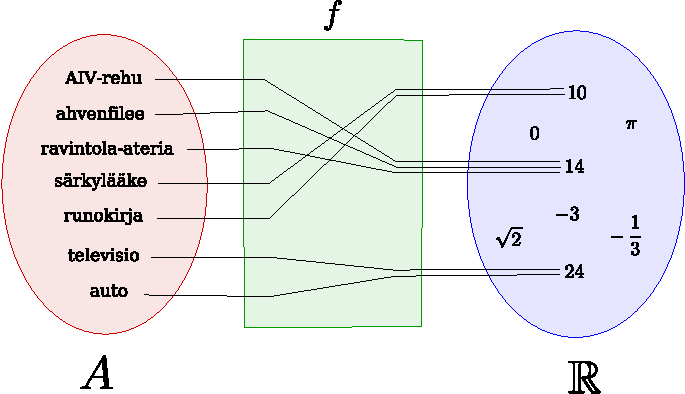
\includegraphics[width=13cm]{pictures/funktiokone.pdf}
	\end{center}
\end{esimerkki}

Funktioiden käyttämiseen liittyy joitakin vakiintuneita tapoja:
\begin{alakohdat}
	\alakohta{$f(x) = y$ lausutaan: ''Funktio saa arvon $y$ pisteessä $x$'',}
	\alakohta{Funktion määrittely- ja maalijoukot jätetään usein merkitsemättä, jos ne voidaan päätellä asiayhteydestä.
		Tällä kurssilla funktiot ovat yleensä reaaliluvuilta reaaliluvuille.}
	\alakohta{Toisinaan funktiolle ja funktion kuvaajalle ei tehdä selkeää eroa:
		$y = f(x)$ samaistetaan koordinaatistoon piirretyn funktion kuvaajan kanssa.
		Periaatteessa funktio ja sen kuvaaja ovat kuitenkin eri asioita.}
\end{alakohdat}

Funktiolla on usein jokin selkeä sääntö, joka voidaan kirjoittaa matemaattisena lausekkeena.

\begin{esimerkki}
	Jos neliön sivun pituutta merkitään muuttujalla $x$, voidaan sivun pituuden
	ja neliön pinta-alan välistä yhteyttä kuvata funktiolla $A(x) = x^2$.
\end{esimerkki}

Funktion määrittelyjoukko koostuu niistä muuttujan arvoista, joilla
funktio on määritelty eli joilla funktion arvo voidaan laskea.

\begin{esimerkki}
	Määritellään funktio $f$ lausekkeella
	\[ f(x) = \frac{1}{x-1}. \]
	Mikä on funktion määrittelyjoukko?
	
	\begin{esimratk}
		Funktio $f(x)$ on määritelty, kun nimittäjä $x-1$ on erisuuri kuin 0.
		Tämä toteutuu kaikilla $x$:n arvoilla lukuun ottamatta arvoa $x = 1$.
		Funktion määrittelyjoukkoon kuuluvat siis kaikki reaaliluvut paitsi luku $1$.
	\end{esimratk}
\end{esimerkki}

Funktion \termi{arvojoukko}{arvojoukko} sisältää ne maalijoukon alkiot,
jotka funktio saa arvokseen ainakin yhdessä pisteessä.

\begin{esimerkki}
	Mikä on edellä määritellyn funktion $f(x)$ arvojoukko?
	% ratkaisu tarvitsee korjausta?
	\begin{esimratk}
		Arvojoukon selvittämiseksi tutkitaan, millä luvun $a$ arvoilla
		yhtälöllä $f(x) = a$ on ratkaisu,
		\begin{align*}
			a &= \frac{1}{x-1} & &| \, \text{Oletetaan, että $x \neq 1$, jolloin voimme} \\
			\text{kertoa lausekkeella $(x-1)$ puolittain.} \\
			a(x-1) &= 1 \\
			x-1 &= \frac{1}{a} \\
			x &= 1+\frac{1}{a} & &| \, \text{Havaitaan, että yhtälöllä on ratkaisu kaikilla $a \neq 0$.}
		\end{align*}
		Funktion arvojoukkona on siis koko reaalilukujen joukko poislukien luku $0$.
	\end{esimratk}
\end{esimerkki}

Funktioita reaaliluvuilta reaaliluvuille voidaan havainnollistaa koordinaatistossa kuvaajien avulla. Funktion $f$ kuvaajassa koordinaatistoon piirretään ne pisteet, joilla y-koordinaatti on $f$:n arvo sen x-koordinaatissa. Siis kaikilla $f$:n määrittelyjoukon luvuilla $x$ lasketaan $y = f(x)$ ja piirretään piste $(x, y)$ koordinaatistoon. Funktioita voi piirtää helposti myös graafisilla laskimilla tai tietokoneohjelmilla (esimerkiksi Wolfram Alphalla\footnote{\url{http://www.wolframalpha.com/}}).

% Tarvitaan kuvien ja taulukkojen vierekkäin laittamiseen.
\def\vcent#1{\mathsurround0pt$\vcenter{\hbox{#1}}$}

\begin{esimerkki}
Funktion $f(x) = \frac{x}{2} - 1$ kuvaaja sisältää kaikki pisteet $(x, y)$, joilla pätee $y = \frac{x}{2} - 1$:
\begin{center}
\begin{tabular}{cc}
\begin{tabular}{|r|l|}
\hline
$x$ & $y = f(x)$ \\
\hline
$-3$ & $-2,5$ \\
$-2$ & $-2$ \\
$-1$ & $-1,5$ \\
$0$ & $-1$ \\
$1$ & $-0,5$ \\
$2$ & $0$ \\
$3$ & $0,5$ \\
\hline
\end{tabular} &
\vcent{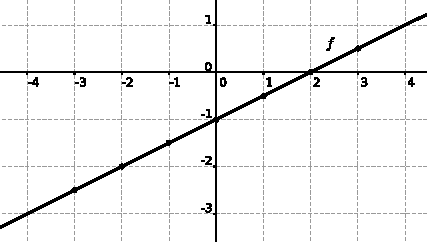
\includegraphics[width=8cm]{pictures/suoraesim.pdf}}
\end{tabular}
\end{center}
\end{esimerkki}

\begin{esimerkki}
Funktion $f(x) = x^2$ kuvaaja sisältää kaikki pisteet $(x, y)$, joilla pätee $y = x^2$:
\begin{center}
\begin{tabular}{cc}
\begin{tabular}{|r|l|}
\hline
$x$ & $y = f(x)$ \\
\hline
$-2$ & $4$ \\
$-1$ & $1$ \\
$-0,5$ & $0.25$ \\
$0$ & $0$ \\
$0,5$ & $0.25$ \\
$1$ & $1$ \\
$2$ & $4$ \\
\hline
\end{tabular} &
\vcent{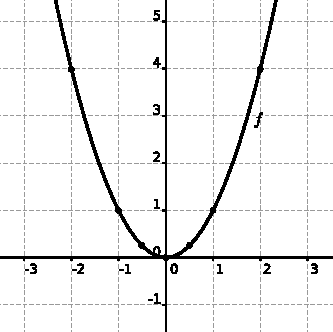
\includegraphics[width=6cm]{pictures/paraabeli.pdf}}
\end{tabular}
\end{center}
\end{esimerkki}

\begin{esimerkki}
Funktion $f(x) = x^3-5x+2$ kuvaaja sisältää kaikki pisteet $(x, y)$, joilla pätee $y = x^3-5x+2$:
\begin{center}
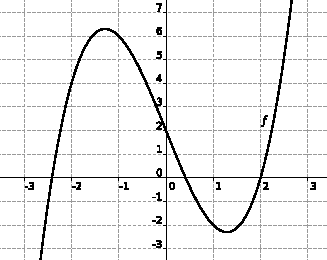
\includegraphics[width=7cm]{pictures/deg3polynomiesim.pdf}
\end{center}
\end{esimerkki}
